\lhead{Capítulo \ref{ch_1}}
\rhead{\newtitle}
\cfoot{\thepage}
\renewcommand{\headrulewidth}{1pt}
\renewcommand{\footrulewidth}{1pt}

\chapter{Marco teórico}\label{ch_1}
\section{Contexto}
\noindent El término ``experimentación con animales'' se refiere a los procedimientos realizados en animales vivos con propósitos de investigación o para realizar pruebas de eficacia a diversos productos de la industria farmacéutica.\\

\noindent Se estima que más de 115 millones de animales en todo el mundo se utilizan en experimentos de laboratorio cada año. Pero debido a que solo una pequeña proporción de países recopila y publica datos sobre el uso de animales para pruebas e investigaciones, se desconoce el número exacto. Por ejemplo, en los Estados Unidos, hasta el 90 por ciento de los animales utilizados en los laboratorios (ratas, ratones y pájaros criados a propósito, peces, anfibios, reptiles e invertebrados) están excluidos de las estadísticas oficiales, lo que significa que las cifras publicadas por el Departamento de Agricultura de los Estados Unidos son sin duda una subestimación sustancial.\\

\noindent Otro ejemplo es la Unión Europea, donde se utilizan más de 12 millones de animales cada año, siendo Francia, Alemania y el Reino Unido los países que más usan animales.
Durante casi un siglo, las evaluaciones de seguridad de medicamentos y productos químicos se han basado en pruebas de laboratorio con roedores, conejos, perros y otros animales. Además de los problemas éticos que plantean (que infligen tanto dolor físico como sufrimiento psicológico), las pruebas con animales también tienen problemas como que requieren de mucho tiempo y recursos, limitan la cantidad de sustancias que se pueden analizar, proporcionan poca comprensión de cómo se comportan los productos químicos en el cuerpo y, en muchos casos, no predicen correctamente las reacciones humanas en el mundo real.\cite{1}\\

\noindent Dichos problemas también se aplican al desarrollo de nuevos fármacos. El alto costo y la gran cantidad de recursos necesarios para este ejercicio se deben en gran parte a la estricta regulación que rige este proceso, así como a los muchos pasos necesarios para descubrir, probar, fabricar y comercializar el nuevo medicamento.\\

\noindent Antes de que se descubra una nueva medicina potencial, los científicos estudian la enfermedad de interés y caracterizan moléculas importantes, principalmente proteínas, que juegan un papel crucial en la enfermedad. Una de las ideas centrales en el descubrimiento de fármacos es evitar de alguna manera que estas proteínas lleven a cabo su función, alterando así el curso de la enfermedad. Esto se puede hacer usando otras moléculas más pequeñas (los medicamentos) que se unen a las proteínas y evitan que la enfermedad progrese.\\

\noindent La búsqueda de estos medicamentos involucra robots y computadoras que pueden probar físicamente cientos de miles de moléculas. Las mejores moléculas resultantes de esta búsqueda se llaman hits. Los principales hits se estudian para garantizar que no sean tóxicos y que puedan llegar al sitio de la proteína dentro del cuerpo humano. Más tarde, los hits se optimizan aún más para que sean más efectivos y seguros.\\

\noindent Las computadoras se utilizan en cada paso de este proceso de trabajo intensivo. El software de la computadora se usa para reducir la cantidad de moléculas a analizar, para simular el efecto del medicamento en el cuerpo (como la toxicidad) y para estudiar y ajustar las propiedades moleculares que aumentan la efectividad del medicamento.\cite{2}\\

\section{Presencia de las tecnologías}
\noindent En la actualidad, la presencia de la tecnología en el área de las ciencias médico-biológicas ha cambiado por completo la trayectoria para el desarrollo de los fármacos, identificando y descubriendo nuevas soluciones potenciales con una reducción significativa de costos y tiempo.\\

\noindent Con el paso del tiempo, se ha desarrollado el conocimiento de la composición molecular, las características estructurales, la disposición y las propiedades de los productos farmacéuticos, y las computadoras se han convertido en una parte esencial al actuar como una herramienta de documentación, análisis y representación.\\

\noindent Una de las disciplinas que tienen más presencia en la inmersión tecnológica a los procesos de las ciencias médico-biológicas, es la Bioinformática.
\subsection{Bionformática}
\subsubsection{Introducción a la Bioinformática}
\noindent La Bioinformática es un área de investigación interdisciplinaria en la interfaz entre la Informática y la Ciencia Biológica.
En la revista científica Methods of Information in Medicine\cite{3}, los autores definen a la Bioinformática como la unión de la biología con la informática: Esta área de estudio implica el uso de la tecnología y utiliza las computadoras para el almacenamiento, recuperación, manipulación y distribución de información relacionada con macromoléculas biológicas tales como ADN, ARN y proteínas. El énfasis aquí está en el uso de computadoras debido a que la mayoría de las tareas en el análisis de datos genómicos son altamente repetitivas o matemáticamente complejas.\\
\subsubsection{Diseño de fármacos asistido por computadora}
\noindent La Bioinformática juega un papel principal en el descubrimiento de fármacos. Este proceso puede llegar a ser complejo y costoso, y en él convergen diversas áreas del conocimiento. En años recientes se han ido incorporando métodos computacionales que entre otras cosas, han contribuido al análisis eficiente de datos, el filtrado colecciones de compuestos para seleccionar moléculas para evaluación experimental, la generación de hipótesis para ayudar a entender el mecanismo de acción de fármacos y el diseño de nuevas estructuras químicas.\\

\noindent Entonces, lo que hoy se conoce como diseño farmacéutico asistido por computadora (CADD, por sus siglas en inglés) contempla en sus avances la reducción del uso de animales para la experimentación, la asistencia para el diseño de fármacos más efectivos y para reposicionar medicamentos conocidos, ayudando a los químicos medicinales en cada paso (diseño, descubrimiento, desarrollo y optimización de la precisión) durante el proceso de descubrimiento de medicamentos. Todo esto a la par de dos panoramas: primero, que los métodos convencionales para el descubrimiento de fármacos implican la detección aleatoria costosa de compuestos sintetizados o productos naturales. Segundo, los procedimientos computacionales pueden ser muy diversos y requieren estudios interdisciplinarios y la aplicación de la informática para diseñar racionalmente medicamentos efectivos y comercialmente factibles.\cite{4}\\

\subsubsection{Los experimentos \textit{in silico}}
\noindent Y si se habla del diseño y descubrimiento de nuevos fármacos, se debe mencionar a la experimentación \textit{in silico}. Los experimentos \textit{in silico} hacen referencia a la simulación, modelado y visualización de procesos médicos y biológicos por medio de computadoras, permitiendo realizar predicciones y simulaciones, con la máxima precisión, de procesos biológicos reales en un entorno virtual \cite{5}. Esta manera de realizar experimentos se presenta como una alternativa para los métodos convencionales que son utilizados en la actualidad: la experimentación in-vivo (uso de ejemplares vivos) y la experimentación in-vitro (uso de partes de organismos que han sido aislados de su entorno biológico natural). La experimentación in-silico a su vez posee varios métodos con los que puede implementarse, unos con más aceptación que otros. Estos métodos son\cite{6}:\\

- Modelado de homología: El modelado de homología (también conocido como modelado comparativo) de proteínas, es un método que permite generar un modelo desconocido de resolución atómica de la proteína ``objetivo'' a partir de su secuencia de aminoácidos y una estructura tridimensional experimental (3D) de una proteína homóloga relacionada (la ``plantilla'').\\

- Acoplamiento molecular (redes de interacción): En el campo del modelado molecular, el “acoplamiento (docking) es una técnica que prevé la orientación preferida de una molécula a una segunda, cuando se unen entre sí para formar un complejo estable. El acoplamiento molecular denota la unión del ligando a su receptor o proteína objetivo. El acoplamiento molecular se utiliza para reconocer y optimizar los candidatos a fármacos al examinar y modelar las interacciones moleculares entre el ligando y las macromoléculas objetivo.\\

- Screening virtual de alto rendimiento: es una técnica computacional en la que se evalúa el potencial de grandes bibliotecas de compuestos para enlazarse a sitios específicos en moléculas objetivo como las proteínas. La investigación en el proceso de descubrimiento de fármacos implica el uso de Virtual Screening (VS), que es un método computacional utilizado para la exploración rápida de grandes bibliotecas de estructuras químicas con el fin de identificar aquellas estructuras que tienen más probabilidades de unirse a un fármaco objetivo, generalmente un receptor de proteínas o enzima. Esta técnica actualmente juega un papel vital en el proceso de descubrimiento de fármacos.\\

- Quantitative structure-activity relationships (QSAR): Las relaciones estructura-actividad cuantitativas (QSAR, por sus siglas en inglés) agrupan un conjunto de métodos que se utilizan para mostrar una relación de descriptores estructurales y / o de propiedades de los compuestos con sus actividades biológicas. Estos descriptores que explican las propiedades estéricas, topológicas, electrónicas e hidrofóbicas de numerosas moléculas, se han determinado mediante métodos empíricos, y son lo más recientemente mediante métodos computacionales.\\

- Hologram quantitative structure activity relationship (HQSAR): En formato de holograma, las relaciones estructura-actividad de holograma (HQSAR, por sus siglas en inglés) no precisan de información en 3D acerca de los ligandos. En este método, la molécula se fragmenta en una huella molecular codificando la frecuencia de ocurrencia para varios tipos de fragmentos moleculares. Sencillamente, la longitud mínima y máxima de los fragmentos depende de el tamaño del mismo que será incluido en la huella de holograma.\\

- Análisis de campo molecular comparativo: Este análisis (abreviado en inglés CoMFA) es una técnica constructiva para explicar la relación estructura - actividad. Si bien su desarrollo comenzó junto con el de QSAR en los años 70’s, actualmente no se ha indagado mucho en esta técnica debido al éxito que ha representado QSAR.\\

- Mapeo farmacóforo en 3D: Este método, simple e imperativo, procede a reconocer fácilmente lo compuestos potenciales junto con un objetivo preferido. Un farmacóforo se define como un conjunto específico en 3D de grupos funcionales en un marco molecular que son indispensables para unirse a un sitio activo de una enzima o para congeniar con un macromolécula. Una vez que este farmacóforo ha sido reconocido, el químico utiliza las herramientas de búsqueda de bases de datos 3D para recuperar nuevos compuestos que son adecuados para el modelo de farmacóforo.\\

- Análisis de micro-conjuntos: Esta es una técnica relativamente nueva, conocida como tecnología ADN que juega un rol muy importante en los avances biotecnológicos. Son básicamente conjuntos propiamente ordenados de una secuencia conocida de moléculas de ADN . Mayormente rectangulares, pueden ser construidas con cientos o miles de conjuntos. Cada característica individual se maneja en la matriz en la posición demarcada con precisión en el sustrato. La identidad de la molécula de ADN asociada a cada característica definitivamente no cambia. Los científicos usan esta información para conocer los resultados de sus experimentos. El estudio de micro conjuntos ayuda a los científicos a percibir inmediatamente numerosos genes en una pequeña muestra y también a llevar a cabo el análisis de la expresión de estos genes.\\

- Análisis conformacional: El análisis conformacional trata con moléculas deformables y sus configuraciones de energía mínima a través de varios métodos de cálculo y redes de interacción implica comparar un sitio del receptor molecular de otra molécula y calcular la conformación tridimensional más satisfactoria energéticamente.\\

- Simulación de Monte Carlo: Los principios de la mecánica estadística están involucrados en la simulación de Monte Carlo, que produce diferentes conformaciones adecuadas de un sistema mediante simulación por computadora para permitir que las propiedades termodinámicas, estructurales y numéricas preferidas se calculen como un promedio ponderado de estas propiedades sobre estas conformaciones.\\

- Simulación de molecular dynamics (MD): La dinámica molecular es un procedimiento efectivo y depende de la simulación del movimiento molecular resolviendo las ecuaciones de movimiento de Newton para cada átomo y aumentando la velocidad y la posición de cada átomo mediante un pequeño aumento de la duración del tiempo. Las simulaciones de MD caracterizan métodos alternativos para muestrear el espacio de configuración, en base a la regla mencionada anteriormente.\\

\subsubsection{QSAR}
\noindent QSAR es una metodología  que relaciona numéricamente estructuras (químicas) con sus actividades biológicas. Esta metodología reúne un conjunto de modelos computacionales relacionados con el diseño, la visualización espacial, la virtualización de moléculas y el cálculo de sus propiedades fisicoquímicas, mediante la Bioinformática y la Estadística. Todo esto con el objetivo de hacer una predicción de la actividad biológica referente a los compuestos seleccionados, que permita el diseño teórico de posibles nuevos fármacos, evitando pasar por el proceso de prueba y error de la síntesis orgánica.\\

\noindent Para llevar a cabo un estudio de tipo QSAR se necesitan básicamente tres tipos de información: (A) Estructura molecular de diferentes compuestos; (B) Datos de actividad biológica de cada uno de los ligandos incluidos en el estudio (opcional) y (C) Propiedades fisicoquímicas (descriptores numéricos) de los ligandos calculados por medios computacionales a partir de la estructura molecular generada in sílico.\cite{7}\\

\noindent De manera general se puede considerar que un modelo básico de QSAR utiliza las estructuras moleculares de los compuestos y sus propiedades fisicoquímicas para realizar el procedimiento de predicción de las actividades biológicas de dichos compuestos frente a la patología, aunque nunca está de más información adicional como los mecanismos de acción de los fármacos o sus actividades biológicas individuales, que proporcionan más robustez al modelo y mejoran el porcentaje de exactitud de la predicción.\\

\noindent La figura\ref{figura1} da una vista general del proceso de QSAR y muestra un ejemplo sencillo de los pasos a seguir para obtener las actividades biológicas de un conjunto inicial de compuestos.\\

\begin{figure}[H]
    \centering
    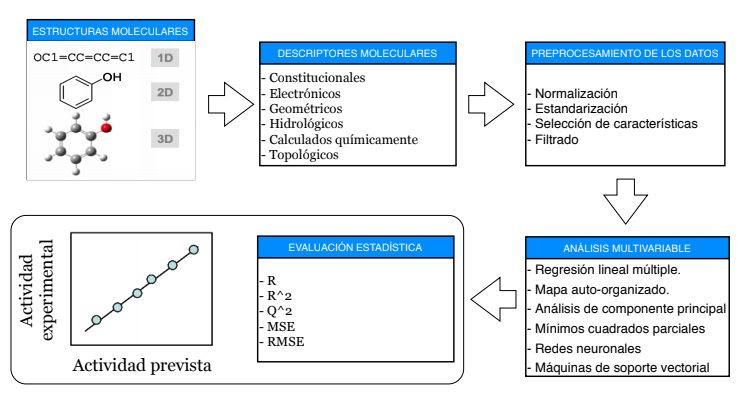
\includegraphics[scale=0.45]{Capitulo1/figuras/figura1.png}
    \caption{Pasos a seguir para realizar el modelado por QSAR.}
    \label{figura1}
\end{figure}
\noindent De la figura anterior se definen a los compuestos, de acuerdo con la Encyclopedia Britannica, como cualquier sustancia compuesta de moléculas idénticas que consisten en átomos de dos o más elementos químicos.\cite{8}\\

\noindent Para obtener la información de los compuestos y sus respectivas estructuras moleculares, se utiliza DrugBank. DrugBank es una base de datos en línea completa y de libre acceso que contiene información sobre fármacos. Como un recurso bioinformático y químico-informático, DrugBank combina datos detallados de medicamentos (es decir, químicos, farmacológicos y farmacéuticos) con información completa sobre el objetivo del medicamento (es decir, secuencia, estructura y vía).\\

\noindent Luego los descriptores moleculares pueden definirse como la información esencial de una molécula en términos de sus propiedades fisicoquímicas (constitución, electrónica, geométrica, etc) de acuerdo con el artículo\textit{ A PRACTICAL OVERVIEW OF QUANTITATIVE STRUCTURE - ACTIVITY RELATIONSHIP} de la revista en línea para las ciencias experimentales y clínicas (\textit{EXCLI}, por sus siglas en inglés)\cite{9}.\\

\noindent La información referente a los descriptores se obtiene utilizando PubChem. PubChem es una base de datos de moléculas químicas y sus actividades contra ensayos biológicos. El sistema es mantenido por el Centro Nacional de Información Biotecnológica (NCBI, por sus siglas en inglés), un componente de la Biblioteca Nacional de Medicina (NLM, por sus siglas en inglés), que forma parte de los Institutos Nacionales de Salud (NIH, por sus siglas en inglés) de los Estados Unidos.
En ese mismo artículo se habla sobre los módulos restantes de la figura \ref{figura1}, que se detallan a continuación.\\

\noindent En el apartado del preprocesamiento de los datos, cuando se obtiene la información sobre los compuestos y sus descriptores, se advierte que dicha información puede tener inconsistencias, por eso, para realizar un análisis preciso, se debe “limpiar” y dejar un conjunto de datos mejorado.\\

\noindent Luego, el módulo denominado análisis multivariante define esencialmente un enfoque para discernir cuantitativamente las relaciones entre las variables independientes (p. ej., descriptores moleculares) y las variables dependientes (p. ej., actividades biológicas de interés).\\

\noindent Ahora, para un modelo QSAR robusto es necesario validar el modelo así como aplicar parámetros estadísticos para evaluar su rendimiento predictivo. Esto se hace en el módulo de evaluación estadística.\\

\noindent Finalmente, como resultado de todos los módulos mencionados anteriormente, se obtiene la información acerca del comportamiento (por predicción) de un conjunto de datos (fármacos) frente a cierta patología (proteínas).\\

\noindent La metodología QSAR es interdisciplinaria, por lo que recibe información de la Química Orgánica y de la Farmacología. En concreto, QSAR persigue el diseño molecular dirigido de compuestos con potencial farmacológico, permitiendo el ahorro de recursos económicos y humanos.\\

\noindent Una de las ventajas más notables en el uso de QSAR es el hecho de que al ser una ciencia que existe sólo en un entorno virtual – desmaterializado de necesidades de infraestructura (tales como equipo, instrumentos, materiales y personal de laboratorio) – con enfoque en las relaciones estructura (química) – actividad (biológica), el diseño de candidatos a nuevos fármacos es mucho más económico y rápido. En cuanto a sus desventajas están la familiarización con metodologías computacionales (diferentes sistemas operativos e interfaces gráficas, manejo de bases de datos, desarrollo del software) y en este sentido, la resolución de diferentes problemas de cómputo (compatibilidad, actualizaciones, registros, formatos de datos) así como el hecho de tener que disponer de datos de actividad biológica de las moléculas que provengan de una misma fuente.\\

\subsubsection{\textit{Machine Learning}}
\noindent El término de \textit{Machine Learning}, hace referencia a lograr que una máquina aprenda sin programarlas explícitamente, para esto existen 4 métodos generales, los cuales son:\\

\noindent- Supervisado.\\
- No supervisado.\\
- Semi-supervisado.\\
- Refuerzo de aprendizaje.\\

\noindent Siendo así, los objetivos de \textit{Machine Learning} consisten en lograr que máquinas sean capaces de realizar predicciones, realizar agrupamiento de conjuntos, tomar decisiones a partir de un conjunto de datos, u obtener reglas de asociación.\cite{10}\\

\noindent \textit{Machine Learning} tiene un gran vínculo  con la optimización   muchos problemas de aprendizaje se formulan como la minimización de alguna función de pérdida en un conjunto de ejemplos de capacitación. Las funciones de pérdida expresan la discrepancia entre las predicciones del modelo que se está entrenando y las instancias del problema real (por ejemplo, en la clasificación, uno quiere asignar una etiqueta a las entradas, y los modelos están entrenados para predecir correctamente las etiquetas preasignadas de un conjunto de ejemplos).\\
\section{Métodos de \textit{Machine Learning}}
\subsection{Árbol de decisión de aprendizaje}
\noindent Un árbol tiene muchas analogías en la vida real, y resulta que ha influido en un área amplia del aprendizaje automático, cubriendo tanto la clasificación como la regresión. En el análisis de decisiones, se puede usar un árbol de decisiones para representar visual y explícitamente las decisiones y la toma de decisiones. Como su nombre indica, utiliza un modelo de decisiones en forma de árbol.
En resumen se dibuja un árbol de decisión al revés con su raíz en la parte superior. Se tiene una condición / nodo interno, en función del cual el árbol se divide en ramas/bordes. El final de la rama que ya no se divide es la decisión(hoja).\\

\noindent Sin embargo, un conjunto de datos real tendrá muchas más funciones y esto solo será una rama en un árbol mucho más grande, pero no puede ignorar la simplicidad de este algoritmo. La importancia de la característica es clara y las relaciones se pueden ver fácilmente. Esta metodología se conoce más comúnmente como árbol de decisión de aprendizaje de los datos y el árbol anterior se llama árbol de clasificación, ya que el objetivo es clasificar a los pasajeros como sobrevivientes o fallecidos. Los árboles de regresión se representan de la misma manera, solo predicen valores continuos como el precio de una casa. En general, los algoritmos del Árbol de decisión se denominan CART o Árboles de clasificación y regresión.\\
%%%%%%%%%%%%%%%%%%%%%%%%%%%%%%%%%%%%%%%%%%%%%%%%55
\subsection{Redes Neuronales Artificiales}
\noindent Un algoritmo de aprendizaje de la red neuronal artificial (RNA), generalmente llamado ``red neuronal'' (RN), es un algoritmo de aprendizaje inspirado en la estructura y los aspectos funcionales de las redes neuronales biológicas. Los cálculos se estructuran en términos de un grupo interconectado de neuronas artificiales, que procesan la información utilizando un enfoque conexionista para el cálculo\cite{11}. Las redes neuronales modernas son herramientas de modelado de datos estadísticos no lineales. Por lo general, se usan para modelar relaciones complejas entre entradas y salidas, para encontrar patrones en los datos o para capturar la estructura estadística en una distribución de probabilidad conjunta desconocida entre las variables observadas.
%%%%%%%%%%%%%%%%%%%%%%%%%%%%%%%%%%%%%%%%%%%%%%
\subsection{Máquina  de Soporte Vectorial (SVM)}
\noindent La Máquina de Soporte Vectorial es otro algoritmo simple que todo experto en aprendizaje automático debería tener en su arsenal. La máquina de vectores de soporte es muy preferida por muchos, ya que produce una precisión significativa con menos potencia de cálculo. Maquina de Soporte Vectorial, abreviado como SVM por sus siglas en inglés, se puede usar tanto para tareas de regresión como de clasificación. Pero, es ampliamente utilizado en los objetivos de clasificación. El objetivo del algoritmo de máquina de vectores de soporte es encontrar un hiperplano en un espacio N-dimensional (N - el número de características) que clasifica claramente los puntos de datos.\\

\noindent Para separar las dos clases de puntos de datos, hay muchos hiperplanos posibles que podrían elegirse. Nuestro objetivo es encontrar un plano que tenga el margen máximo, es decir, la distancia máxima entre los puntos de datos de ambas clases. Maximizar la distancia de margen proporciona cierto refuerzo para que los puntos de datos futuros se puedan clasificar con más confianza\cite{12}.\\
%%%%%%%%%%%%%%%%%%%%%%%%%%%%%%%%%%%%%%%%%%%%%%%%%%%%
\subsection{Aprendizaje por refuerzo}
\noindent El Aprendizaje por refuerzo se refiere a cómo un agente debe tomar medidas en un entorno para maximizar alguna noción de recompensa a largo plazo. Los algoritmos de aprendizaje por refuerzo intentan encontrar una política que asigne estados del mundo a las acciones que el agente debe tomar en esos estados. El aprendizaje de refuerzo difiere del problema de aprendizaje supervisado en que los pares de entrada / salida correctos nunca se presentan, ni las acciones subóptimas se corrigen explícitamente.\\

\noindent El aprendizaje de refuerzo, debido a su generalidad, se estudia en muchas otras disciplinas, como la teoría de juegos, la teoría de control, la investigación de operaciones, la teoría de la información, la optimización basada en simulación, los sistemas de múltiples agentes, la inteligencia de enjambre, las estadísticas y los algoritmos genéticos. En la literatura de investigación y control de operaciones, el aprendizaje por refuerzo se denomina programación dinámica aproximada o programación neurodinámica.\\

%%%%%%%%55
\section{\textit{Machine Learning} en la Bioinformática}
\noindent \textit{Machine Learning} se ha convertido en uno de los temas que más se ha desarrollado, siendo muy útil para el descubrimiento de nuevos fármacos asistidos por computadora, esto ya que \textit{Machine Learning} aprovecha el uso de algoritmos para la clasificación y reconocimientos de patrones, aprovecha estas bases para predecir propiedades físicas, químicas incluso biológicas de nuevos compuestos. Otra enorme ventaja es la gran eficiencia para la lectura y análisis de gran cantidad de datos sin requerir una vasta cantidad de recursos.  Hoy en día las técnicas de \textit{Machine Learning} pueden ser usadas para el modelado QSAR y así lograr el desarrollo de programas inteligentes con la capacidad de predecir por in-silico la forma en que modificaciones químicas pueden influir en el comportamiento biológico.\\

\noindent Gracias a esto actualmente hay gran cantidad de aplicaciones y estudios de la Bioinformática, pues la principal meta de estas técnicas es adquirir exitosamente información útil por medio de la elaboración de abstracción probabilística.  En general consiste en programas computacionales, para optimizar un proceso utilizando algún dato como ejemplo o experiencia previamente adquirida.\\

\noindent De acuerdo con un artículo del Diario de Química Medicinal recuperado por el Centro Nacional de Información Biotecnológica de los Estados Unidos, el aumento de las medidas para regular la producción y venta de productos químicos, así como la reducción de recursos para las pruebas de dichos productos, han hecho que los modelos de QSAR se utilicen cada vez más en la detección, la priorización de pruebas, las iniciativas de prevención de la contaminación, la química ecológica, la identificación de peligros y la evaluación de riesgos. Sin embargo, para ser aceptados por los usuarios finales (toxicólogos, reguladores, industria), estos QSAR deben cumplir con una gama de necesidades, incluida la relevancia para los esquemas regulatorios, la transparencia, la plausibilidad biológica y la comprensión por parte de los no desarrolladores.\\

\noindent La revista Future-Science, en el artículo Current trends in quantitative structure–activity relationship validation and applications on drug discovery, menciona que Las técnicas de \textit{Machine Learning} se han empleado ampliamente en el campo QSAR para construir modelos de regresión y clasificación utilizando grandes conjuntos de datos de dominio público y / o utilizando conjuntos grandes que contienen descriptores calculados

%%%%%%%%%%%%%%%%%%%%%%%%%%%%%%%%%%%%%%%%%%%%%5
\section{Alternativas de solución}
\noindent En la actualidad, los métodos de \textit{Machine Learning} y la metodología de QSAR permiten tener una visión más novedosa y menos egoísta hacia la experimentación, en la cual se haga uso de las ventajas que ofrece la tecnología para realizar este proceso involucrando el menor número de animales posible.
Es por ello que tanto \textit{Machine Learning} como QSAR pueden enfocarse al ámbito del diseño de fármacos asistido por computadora para construir un sistema que realice el proceso de la experimentación científica con mayor rapidez, obteniendo mejores resultados, y reduciendo el uso de seres vivos para dicho proceso.\\

\noindent De hecho, sistemas como el que se propuso anteriormente ya existen. Cabe destacar que debido a la cantidad de información que puede arrojar el análisis de grado molecular de una bacteria (sin mencionar virus, hongos, etc.), las soluciones actuales que se presentan, hacen uso el uso de métodos \textit{in silico} ó \textit{in vitro} y normalmente se enfocan a un área de la medicina en particular (cardiología, oftalmología, etc.)\\

\noindent Un ejemplo es el software Virtual Assay, desarrollado por la Universidad de Oxford, que provee un marco de trabajo para realizar pruebas in-silico en poblaciones de modelos de células cardíacas humanas para predicciones de seguridad y eficacia de fármacos.\\

\noindent Organs-on-chips diseñados por el Instituto Wyss de Harvard, en donde se han adaptado los métodos de fabricación de microchips de computadora para diseñar dispositivos de cultivo de microfluidos que recapitulan la microarquitectura y las funciones de los órganos humanos vivos.\\

\noindent Los modelos de tejido vendidos por MatTek, que son sistemas micro-fisiológicos de los tejidos epiteliales humanos en modelos 3D de tejidos vivos y metabólicamente activos que permiten a los investigadores la flexibilidad de los experimentos agudos o a largo plazo en un entorno altamente fisiológico e in vitro y que se basan en el concepto de sustituir las pruebas en animales.\\

\noindent En la tabla \ref{productos1} se detalla a cada uno de los ejemplos mencionados, incluyendo a la solución propuesta.
Además de estos ejemplos, existen otros más que si bien entran en la categoría de alternativas ya existentes al problema planteado, se encuentran aún en desarrollo, tienen un enfoque diferente al presentado en este documento o solo fueron trabajos meramente académicos.\\

\noindent Software como TOPKAT, enfocado a la toxicología, que explota la estructura molecular de un compuesto para medir y aprobar evaluaciones de sus efectos tóxicos y ambientales, o la aplicación VEGA, que ofrecer una familia de herramientas para evaluar el peligro químico de cierto compuesto son solo algunos de ellos. En la tabla \ref{productos2} se encuentra una lista completa con toda la información de estos y más ejemplos de software para el modelado .\cite{13}

\begin{longtable}{|c|l|c|}
\caption{Resumen de productos similares.}
\label{productos1}\\
\hline
SOFTWARE & \multicolumn{1}{c|}{CARACTER\'iSTICAS} & PRECIO EN EL MERCADO \\ \hline
\endfirsthead
%
\multicolumn{3}{c}%
{{\bfseries Tabla \thetable\ Continuación de la página anterior.}} \\
\hline

\endhead
%
\textit{Virtual Assay} & \begin{tabular}[c]{@{}l@{}}- Marco de trabajo para la\\   realizaci\'on de experimentos por\\   medio del modelado por\\   computadora.\\   - Enfocado a la cardiolog\'ia.\\   - Su m\'etodo de trabajo es el\\    ajuste de modelos   \\   celulares comparados con\\    experimentaciones previas.\end{tabular} & NO COMERCIAL \\ \hline
\textit{Organs-on-Chips} & \begin{tabular}[c]{@{}l@{}}- Se basa en el uso de c\'elulas\\    vivas, adaptadas en pequeños\\   chips.\\   - Permiten la observaci\'on de las\\   c\'elulas humanas y su reacci\'on\\    ante enfermedades espec\'ificas.\\   - Es un m\'etodo in-vitro,\\    no involucra el uso de un \\   software.\end{tabular} & \begin{tabular}[c]{@{}c@{}}\$2,495 USD por placa\\ (6 chips).\end{tabular} \\ \hline
\textit{\begin{tabular}[c]{@{}c@{}}Modelos de tejido \\ MatTek's\end{tabular}} & \begin{tabular}[c]{@{}l@{}} - Son modelos de tejido 3D\\    vivos y metab\'olicamente \\   activos.\\   - Es un m\'etodo in-vitro.\\   - Actualmente tiene modelos\\    para pruebas oculares,\\   dermatol\'ogicas, intestinales y\\   genitales.\end{tabular} & SIN INFORMACIÓN \\ \hline
\textit{Soluci\'on propuesta} & \begin{tabular}[c]{@{}l@{}}- Se basa en el modelado\\    matem\'atico de QSAR.\\   - Es un m\'etodo in-silico.\\   - Utiliza \textit{Machine Learning} \\   para asistir y complementar\\    los resultados de QSAR.\end{tabular} & N/A \\ \hline
\end{longtable}
\begin{longtable}{|c|l|c|}
\caption{Resumen de software académicos o con enfoque diferente al problema planteado.}
\label{productos2}\\

\hline
SOFTWARE & \multicolumn{1}{c|}{CARACTER\'iSTICAS} & PRECIO EN EL MERCADO \\ \hline
\endfirsthead
%
\multicolumn{3}{c}%
{{\bfseries Tabla \thetable\ Continuación de la página anterior.}} \\
\hline

\endhead
%
PASS & \begin{tabular}[c]{@{}l@{}}- Capaz de calcular m\'as\\  de 4000 tipos de\\ actividad biol\'ogica.\\ - Requiere la f\'ormula \\ estructural del\\ compuesto.\\ - Utiliza una base de \\ datos que contiene\\ 260,000 compuestos \\ aproximadamente.\\ - Es comercial.\end{tabular} & NO DISPONIBLE \\ \hline
\textit{TOPKAT} & \begin{tabular}[c]{@{}l@{}}- Enfoque a la toxicidad  de los\\ compuestos.\\ - Modelado utilizando \\ QSTR para el enfoque toxicol\'ogico.\end{tabular} & NO DISPONIBLE \\ \hline
\textit{VEGA hub} & \begin{tabular}[c]{@{}l@{}}- Conjunto de herramientas\\ , enfocadas a la\\ predicci\'on y an\'alisis de la \\ toxicidad de un compuesto.\\ - Una de las herramientas \\ utiliza QSAR para\\ realizar predicciones\end{tabular} & GRATUITO \\ \hline
\textit{Leadscope} & \begin{tabular}[c]{@{}l@{}}- Enfoque en el an\'alisis\\  de toxicidad en\\ una simulaci\'on de los\\  sistemas biol\'ogicos de\\  un roedor.\\ - Utiliza modelos para\\  reproducci\'on,\\ neurotoxicidad, problemas\\  gen\'eticos y agentes\\  cancer\'igenos.\end{tabular} & NO DISPONIBLE \\ \hline
\textit{Derek Nexus} & \begin{tabular}[c]{@{}l@{}}- Enfoque al an\'alisis\\  toxicol\'ogico.\\   - Utiliza su propia \\ base de datos (base\\   privada).\end{tabular} & NO COMERCIAL \\ \hline
ADMET predictor & \begin{tabular}[c]{@{}l@{}}- Se basa en redes\\  neuronales para realizar\\ predicciones ADMET\\  (Absorci\'on, Distribuci\'on,\\  Metabolismo, Eliminaci\'on\\  y Toxicidad) \\ de medicamentos.\\ - Es comercial.\\ - Requiere de un nivel\\  intermedio en habilidades\\  computacionales.\\ - Se enfoca en las \\ propiedades qu\'imicas\\  de los compuestos.\end{tabular} & NO DISPONIBLE \\ \hline
OSIRIS & \begin{tabular}[c]{@{}l@{}}- Realiza an\'alisis de las \\ propiedades\\ f\'isico-qu\'imicas de \\ una mol\'ecula.\\ - Indica beneficios y \\ desventajas acerca de\\ la mol\'ecula estudiada.\\ - La mol\'ecula debe ser \\ construida por el\\ usuario.\end{tabular} & GRATUITO \\ \hline
T.E.S.T. & \begin{tabular}[c]{@{}l@{}}- Utiliza varias metodolog\'ias\\  de QSAR para\\ predicciones toxicol\'ogicas.\\ - Trabaja con la estructura \\ de un compuesto, ya\\ sea en archivo, creado en su \\ herramienta o de una base de\\  datos espec\'ifica.\end{tabular} & GRATUITO \\ \hline
CASE & \begin{tabular}[c]{@{}l@{}}- Capaz de predecir efectos\\  toxicol\'ogicos\\ en animales.\\ - Utiliza el modelo de \\ regresi\'on lineal.\\ - Se encuentra en desarrollo.\end{tabular} & NO DISPONIBLE \\ \hline
LAZAR & \begin{tabular}[c]{@{}l@{}}- Uso de algoritmos\\  estad\'isticos\\  para predecirtoxicidad.\\ - Es un proyecto web.\end{tabular} & GRATUITO \\ \hline
\end{longtable}
\newpage
\section{Arquitectura del sistema}
\noindent Por lo cual, el sistema que se planea desarrollar utilizará la información fisicoquímica y las referencias de experimentaciones previas de un conjunto de fármacos, se realiza una predicción de la actividad biológica de dicho conjunto, utilizando técnicas de \textit{Machine Learning} y QSAR para obtener una medida cuantitativa que permita clasificarlos del más al menos recomendable.\\

\noindent El modelo del sistema está compuesta por tres bloques principales de los cuales podemos clasificar como entradas, proceso y salidas.\\

a)	Entradas.\\

\noindent Las entradas están dadas por una lista de compuestos y una lista de proteínas de la patología, como requerimiento, los nombres de los compuestos y de las proteínas, deberán estar escritas en el idioma ingles para tener una búsqueda eficaz. Con estas listas el sistema puede comenzar la búsqueda de lo siguientes datos: \\

\noindent 1.- Conjunto de compuestos: El sistema recibe datos de diversos compuestos candidatos dados por el usuario, estos interactúan con una proteína perteneciente a una patología, estos datos los obtendremos de la base de datos “DrugBank”.\\

\noindent 2.- Descriptores moleculares: El sistema hará la búsqueda de datos más específicos del conjunto de compuestos previamente mencionados, dichos descriptores poseen información de las propiedades fisicoquímicas, describiendo numéricamente a cada una de las moléculas, estos datos los localizamos en la base de datos “PubChem”.\\

\noindent 3.- Proteínas de la enfermedad: Esta entrada otorga al sistema la información del objeto de estudio, para determinar las actividades biológicas que provocará su interacción con cada uno de los componentes listados en la primera entrada, al igual que en los compuestos, esta información podrá ser localizada en las base de de datos “PDB”.\\

 b)	Procesos.\\
El sistema hará uso de la metodología de QSAR para modelar cada una de las entradas obtenidas y así poder describir numéricamente la molécula, con lo cual el sistema hará  uso de un algoritmo de \textit{Machine Learning} y así poder determinar el resultado de la interacción entre proteína y compuesto, además de que el sistema adquiere la experiencia de esa interacción, para una posible interacción con características similares.\\

c) 	Salidas.\\
Actividad biológica de los compuestos ingresados: El sistema otorgará información y descripción de la actividad biológica causada por el compuesto que haya interactuado con la proteína objetivo, para conocer cuál de los compuestos ingresados obtiene el mejor de los resultados, el sistema generará una lista con dichos resultados que será desplegada al usuario, ordenada del compuesto más apto al menos apto para enfrentar la patología indicada.
\begin{figure}[H]
    \centering
    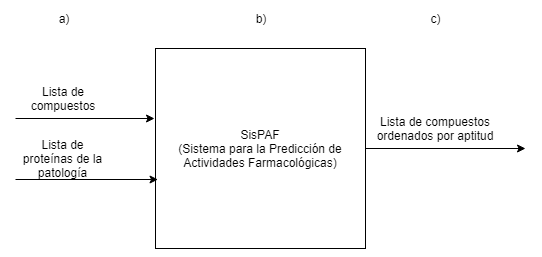
\includegraphics[scale=0.8]{Capitulo1/figuras/arquitectura.png}
    \caption{Arquitectura del sistema}
    \label{arq}
\end{figure}
